%\vspace*{\subsecspace}
%\vspace*{-0.2cm}
\section{Background}

We now give an overview of transient cloud computing, and motivate the need for the bag of jobs abstraction in scientific computing workflows.
%; and give an overview of our \sysname system. 

%\vspace*{\subsecspace}
\subsection{Transient Cloud Computing}
% The "Environment"

Infrastructure as a service (IaaS) clouds such as Amazon EC2, Google Public Cloud, Microsoft Azure, etc., typically provide computational resources in the form of virtual machines (VMs), on which users can deploy their applications.
% too long an opening sentence, not to the point 
Conventionally, these VMs are leased on an ``on-demand'' basis: cloud customers can start up a VM when needed, and the cloud platform provisions and runs these VMs until they are shut-down by the customer. 
%Due to the temporal dynamics of cloud workloads, the overall utilization of cloud platforms is also highly dynamic.
Cloud workloads, and hence the utilization of cloud platforms, shows large temporal variation. 
To satisfy user demand, cloud capacity is typically provisioned for the \emph{peak} load, and thus the average utilization tends to be low, of the order of 25\%~\cite{borg,resource-central-sosp17}. 


To increase their overall utilization, large cloud operators have begun to offer their surplus resources as low-cost servers with \emph{transient} availability, which can be preempted by the cloud operator at any time (after a small advance warning). 
These preemptible servers, such as Amazon Spot instances~\cite{ec2-spot}, Google Preemptible VMs~\cite{preemptible-documentation}, and Azure batch VMs~\cite{azure-batch}, have become popular in recent years due to their discounted prices, which can be 7-10$\times$ lower than conventional non-preemptible servers. 
Due to their popularity among users, smaller cloud providers such as Packet~\cite{packet-spot} and Alibaba~\cite{alibaba-spot} have also started offering transient cloud servers. 


However, effective use of transient servers is challenging for applications because of their uncertain availability~\cite{spotcheck, prateek-thesis}. 
Preemptions are akin to fail-stop failures, and result in loss of the application's memory and disk state, leading to downtimes for interactive applications such as web services, and poor throughput for long-running batch-computing applications. 
Consequently, researchers have explored fault-tolerance techniques such as checkpointing~\cite{flint, marathe2014exploiting, spoton} and resource management techniques~\cite{exosphere} to ameliorate the effects of preemptions. % for a wide range of applications. 
The effect of preemptions is dependent on a combination of application resource and fault model, and mitigating preemptions for different applications remains an active research area~\cite{hourglass-eurosys19}.


%Explain how bags of jobs changes things? 
%Novelty


%In contrast, \sysname can run applications on Google Preemptible VMs that have fixed price and \emph{unknown} preemption rates.
%\vspace*{\subsecspace}
\subsection{Modeling Preemptions of Transient VMs}

% Mainly about spot instances?

Underlying \emph{all} techniques and systems in transient computing is the notion of using some probabilistic or even a deterministic model of their preemptions.
Such a preemption model is then used to quantify and analyze the impact of preemptions on application performance and availability; and to design model-informed policies to minimizing the effect of preemptions.

For example, the preemption rate or MTTF (Mean time to failure) of transient servers has found extensive use in selecting the appropriate type transient server for applications~\cite{exosphere, spoton}, determining the optimal checkpointing frequency~\cite{flint, marathe2014exploiting, proteus-eur17, spark-ckpt-hpdc}, etc.

However, \emph{all} prior work on transient computing has exclusively focused on Amazon's EC2 spot instances.
Launched in 2009, Amazon's EC2 spot instances are the first example of transient cloud servers, and their low price (often 90\% cheaper than equivalent on-demand instances) provided the motivation to develop optimized policies for reducing the impact of preemptions and the overall cost. 

The preemptions of EC2 spot instances are based on their \emph{price}, which is dynamically adjusted based on the supply and demand of cloud resources.
Spot prices are based on a continuous second-price auction, and if the spot price increases above a pre-specified maximum-price, then the server is preempted~\cite{spot-pricing2}.
%
Thus, the time-series of these spot prices can be used for understanding preemption characteristics such as the frequency of preemptions and the ``Mean Time To Failure'' (MTTF) of the spot instances. 
Publicly available\footnotemark historical spot prices have been used to characterize and model spot instance preemptions~\cite{spotcheck, bid-cloud, tr-guarantees}. %Add lots more here 
For example, past work has analyzed spot prices and shown that the MTTFs of spot instances of different hardware configurations and geographical zones range from a few hours to a few days~\cite{wolski_probabilistic_2017, icdcs-spotlight, wolski-new}.

However, using pricing information for preemption modeling is \emph{not} a generalizable approach and is not applicable to other types of transient cloud servers such as Google Preemptible VMs and Azure Low-priority batch VMs.
These servers have \emph{flat} pricing, and thus pricing cannot be used to infer preemptions, unlike in the case of EC2.
Moreover, these cloud providers (Google and Azure) do not expose \emph{any} public information about the preemption characteristics.

The total lack of information about the preemption characteristics precludes the vast array of optimizations and systems that have been developed to make transient computing more appealing to different kinds of applications.
Therefore in this paper, we seek to develop the \emph{first} empirical model of preemptions of Google Preemptible VMs~\cite{pvm}.
Our empirical data and preemption model allows the development of preemption mitigation policies.
%

Google Preemptible VMs have a maximum lifetime of 24 hours, and this \emph{constrained} preemption introduces new challenges in preemption modeling.
Past work on failure modeling of EC2 spot instances have assumed preemptions to be \emph{memoryless} and follow the exponential distribution.
However, the 24 hour constraint precludes such memoryless assumptions, and as we see in the next section, require new modeling techniques.  




% Past work on transient computing has almost exclusively focused on the Amazon EC2 spot market, which has a radically different preemption model and dynamics compared to other transient cloud servers such as those offered by Google Cloud and Azure. 

% \prat{sigcomm paper} 

\footnotetext{Amazon posts Spot prices of 3 months, and researchers have been collecting these prices since 2010~\cite{bidding4}.}


% However the price-based approach for inferring preemption characteristics is of limited utility.
% Other transient VMs such as those offered by Google and Azure have \emph{flat} pricing, and price-based techniques for preemption modeling and cost optimization are not applicable.
% Furthermore, price-based techniques may be of limited value after Amazon's recent change where preemptions were decoupled with pricing.
% To address this shortcomings, we develop \emph{empirical} preemptions models for transient VMs.
% In particular, we focus on Google Preemptible VMs, whose preemption properties have been unknown so far.
% Additionally, their unique fixed lifetime leads to new challenges for conventional reliability theory models, and requires new modeling techniques, which we develop later in Section~\ref{sec:failmodel}. 

%This is an important point but not relevant for us right now 
%However, pricing based models and the policies based on them are at risk when there are changes in the cloud provider's pricing mechanisms and policies. 
%For instance, Amazon has recently changed the preemption characteristics of spot instances, and servers are now preempted even if the spot price is below the maximum price~\cite{spotweb, bid-change}.
%Thus, spot prices are no longer a completely reliable indicator of preemptions, and preemptions can no longer be inferred from looking at prices alone.
%Therefore, new techniques are required to model preemption dynamics that can supplement the earlier price-based approaches, and we develop these techniques next.


% Thus due to the lack of any historical preemption information and the fundamental differences in the preemption characteristics, techniques such as historical price-based bidding strategies~\cite{bid-cloud}, price-based checkpointing~\cite{marathe2014exploiting, xinhpdc, spoton}, and diversification~\cite{exosphere, spotweb}, are unfortunately largely inapplicable. 
% %
% To address these shortcomings, we develop an empirical model of preemptions in Section~\ref{sec:preemption-dynamics}. 
% This model informs our policies for minimizing cost and running time of scientific computing workloads that are launched as bags of jobs, as described next. 



% \vspace*{\subsecspace}
% \subsection{Scientific Simulation Workloads}
% \prat{Not sure. Probably something on scientific workloads though?}

% % \begin{figure}[t]
% %   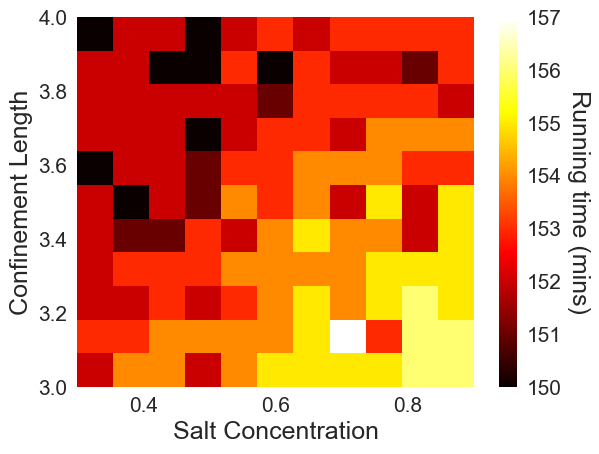
\includegraphics[width=0.3\textwidth]{../graphs/hmap.png}
% %     \vspace*{\myfigspace}
% %   \caption{Running times of the Nanoconfinement application with different sets of parameters have low variation.}
% %   \label{fig:heatmap}
% %   \vspace*{\myfigspace}
% % \end{figure}

% Large computational requirements of scientific simulations make them ideal for low-cost transient servers. 

% The typical workflow associated with most scientific computing applications, often involves evaluating a computational model across a wide range of physical and computational parameters. 
% For instance, constructing and calibrating a molecular dynamics application (such as Nanoconfinement~\cite{jcs2}), usually involves running a simulation with different physical parameters such as characteristic sizes and interaction potentials, as well as computational parameters such as simulation timesteps. 
% Each of these parameters can take a wide range of values, resulting in a large number of combinations which must be evaluated by invoking the application multiple times (also known as a parameter sweep). 
% Since each computational job explores a single combination of parameters, this results in executing a ``bag of jobs'', with each job in the bag running the same application, but with possibly different parameters.


% The bag of jobs execution model is pervasive in scientific computing and applicable in many contexts.
% In addition to exploratory parameter sweeps, bags of jobs also result from running the application a large number of times to account for the model or computational stochasticity, and can be used to obtain tighter confidence intervals. 
% Increasingly, bags of jobs also arise in the emerging research that combines statistical machine learning (ML) techniques and scientific simulations~\cite{ml.atomic2017,melko2017,sam2017}. %,fu2017,long2015machine, ferguson2017machine,ward2018matminer,jcs2,fox2019learning}.
% For instance, large bags of jobs are run to provide the necessary training and testing data for learning statistical models (such as neural networks) that are then used to improve the efficacy of the simulations~\cite{jcs2}.


% Bags of jobs are analogous to, but distinct from the bag of \emph{tasks} design~\cite{bot-2003}, where applications are decomposed into independent processes to enable flexible task scheduling. 
% In contrast, the bags of jobs abstraction is independent of the application design---a bag of jobs may consist of a synchronous MPI program that is not amenable to flexible scheduling. 


% %The bag of jobs resulting from exploratory parameter sweeps are an integral component in the model discovery and validation process, and ar

% %More formally, a bag of jobs is defined as a collection of : \{Application, $N$: Number of jobs, $m$: Minimum number of jobs to finish, $\pi$: Generator function for job parameters, $\mathcal{R}$: Computing resources per job\}

% The bag of jobs execution model has multiple characteristics, that give rise to unique challenges and opportunities when deploying them on transient cloud servers. 
% Since bags of jobs require a large amount of computing resources, deploying them on the cloud can result in high overall costs, thus requiring policies for minimizing the cost and overall running time. 
% The similarity in execution characteristics of jobs (such as their running times and parallel speedup) allows for bag-wide optimizations (Figure~\ref{fig:heatmap}). 
% %Second, there is no dependency between individual jobs in a bag, thus allowing increased flexibility in job scheduling.
% And last, treating entire bags of jobs as an execution unit, instead of individual jobs, can allow us to use partial redundancy between jobs and reduce the fault-tolerance overhead to mitigate transient server preemptions. 



% We will modify our text to safeguard against R2's misunderstanding.
% statistical pattern recognition/machine guessing 
%%% Local Variables:
%%% mode: latex
%%% TeX-master: "paper"
%%% End:
